% ---
% school: "college"
% level: "8eme"
% section: null
% chapter: "التناظر المركزي"
% source: "Axiomaths"
% title: "تحدّي : نقطة منتصف"
% country: "Tunisie"
% year: 2026
% professor: "Axiomaths"
% difficulty: "Difficile"
% points: null
% tags: ["defi", "symetrie-centrale", "cercles", "construction", "milieu"]
% ---
% Exercice 19/19 de la série 8ème « التناظر المركزي » (statement + \axsol + solution). Compiler avec XeLaTeX + axiomath.sty (+ axiomaths-logo.png).
\documentclass[12pt,a4paper]{article}
\usepackage[level=8b,color=15803D]{axiomath}
\usetikzlibrary{arrows.meta}
\newcommand{\cm}{\,\mathrm{cm}}
\axsetup{title={التناظر المركزي}, corrige}

\begin{document}

\begin{corr}[title={تحدّي : نقطة منتصف}, stars=4, source={Axiomaths}]
$\mathcal{C}_1$ و $\mathcal{C}_2$ دائرتان مركزاهما $O_1$ و $O_2$ تتقاطعان في نقطتين $A$ و $B$.
\begin{center}
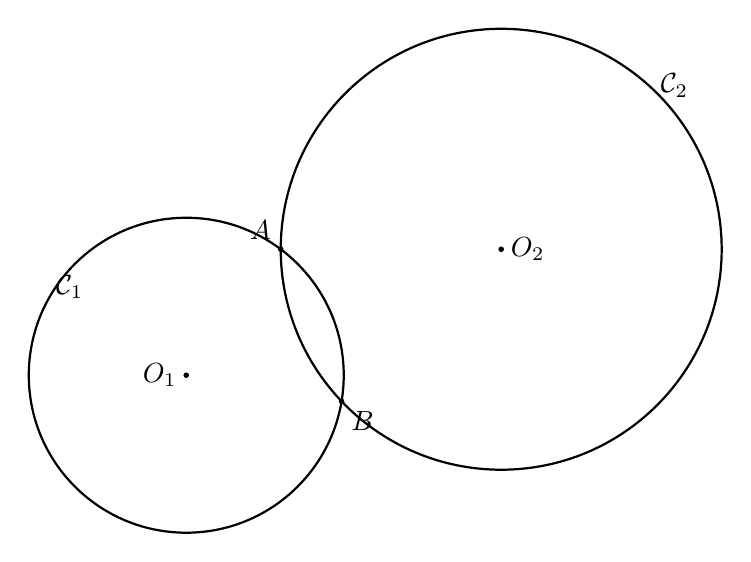
\begin{tikzpicture}[scale=0.4]
  \draw[thick] (-3,-4) circle (5);
  \draw[thick] (7,0) circle (7);
  \fill (0,0) circle (2.5pt) node[above left] {$A$};
  \fill (1.931,-4.828) circle (2.5pt) node[below right] {$B$};
  \fill (-3,-4) circle (2.5pt) node[left] {$O_1$};
  \fill (7,0) circle (2.5pt) node[right] {$O_2$};
  \node at (-6.7,-1.2) {$\mathcal{C}_1$};
  \node at (12.5,5.2) {$\mathcal{C}_2$};
\end{tikzpicture}
\end{center}
نريد رسم مستقيم $\Delta$ يمر من $A$ ويقطع $\mathcal{C}_1$ مرة ثانية في $M$ و $\mathcal{C}_2$ مرة ثانية في $N$ بحيث تكون $A$ منتصف $[MN]$.
\begin{enumerate}
  \item نفترض أن $M$ و $N$ موجودتان. ما هي مناظرة $M$ بالنسبة إلى $A$ ؟ بين أن $N$ تنتمي إلى الدائرة $\mathcal{C}_1'$ مناظرة $\mathcal{C}_1$ بالنسبة إلى $A$.
  \item استنتج طريقة لبناء $N$ ثم $M$ ، ونفّذها على الشكل.
  \item بين أن النقطتين المبنيتين تحققان الشرط المطلوب.
  \item بين أن $\mathcal{C}_1'$ و $\mathcal{C}_2$ لهما نقطة مشتركة ثانية غير $A$ ، وأن المسألة لها حل وحيد. \quad [لماذا لا تكون الدائرتان متماستين في $A$ ؟]
\end{enumerate}
\axsol
\begin{enumerate}[itemsep=14pt]
  \item $A$ منتصف $[MN]$ ، إذن \ib{$N=S_A(M)$}. بما أن $M\in\mathcal{C}_1$ فإن $N=S_A(M)$ تنتمي إلى $S_A(\mathcal{C}_1)=\mathcal{C}_1'$.
  \begin{prop}[مناظرة دائرة]
  مناظرة الدائرة $\mathcal{C}(O\,;r)$ بالنسبة إلى $A$ هي الدائرة $\mathcal{C}'(O'\,;r)$ حيث $O'=S_A(O)$.
  \end{prop}
  إذن $\mathcal{C}_1'$ دائرة مركزها $O_1'=S_A(O_1)$ وشعاعها نفس شعاع $\mathcal{C}_1$. و $N\in\mathcal{C}_2$ أيضا : $N\in\mathcal{C}_1'\cap\mathcal{C}_2$.
  \item \textbf{البناء :}
  \begin{itemize}
    \item نبني $O_1'$ مناظرة $O_1$ بالنسبة إلى $A$ ثم الدائرة $\mathcal{C}_1'$ (مركزها $O_1'$ ، وشعاعها $O_1A$ لأن $A\in\mathcal{C}_1$).
    \item $N$ هي نقطة تقاطع $\mathcal{C}_1'$ و $\mathcal{C}_2$ المختلفة عن $A$.
    \item $\Delta=(AN)$ ، و $M$ مناظرة $N$ بالنسبة إلى $A$.
  \end{itemize}
  \begin{center}
  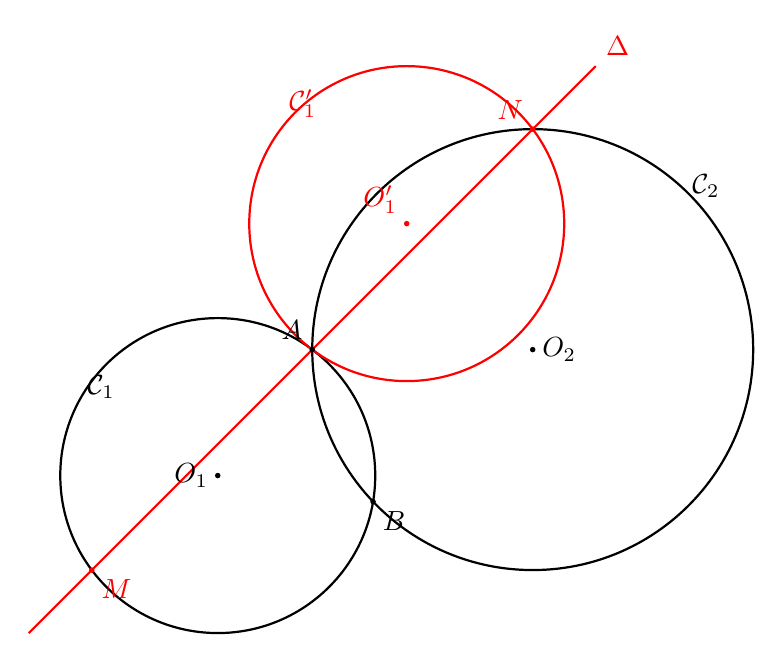
\begin{tikzpicture}[scale=0.4]
    \draw[thick] (-3,-4) circle (5);
    \draw[thick] (7,0) circle (7);
    \draw[thick,red] (3,4) circle (5);
    \draw[thick,red] (-9,-9)--(9,9) node[above right] {$\Delta$};
    \fill (0,0) circle (2.5pt) node[above left] {$A$};
    \fill (1.931,-4.828) circle (2.5pt) node[below right] {$B$};
    \fill (-3,-4) circle (2.5pt) node[left] {$O_1$};
    \fill (7,0) circle (2.5pt) node[right] {$O_2$};
    \fill[red] (3,4) circle (2.5pt) node[above left] {$O_1'$};
    \fill[red] (7,7) circle (2.5pt) node[above left] {$N$};
    \fill[red] (-7,-7) circle (2.5pt) node[below right] {$M$};
    \node at (-6.7,-1.2) {$\mathcal{C}_1$};
    \node[red] at (-0.3,7.8) {$\mathcal{C}_1'$};
    \node at (12.5,5.2) {$\mathcal{C}_2$};
  \end{tikzpicture}
  \end{center}
  \item $N\in\mathcal{C}_1'$ ، فمناظرتها $M=S_A(N)$ تنتمي إلى $S_A(\mathcal{C}_1')=\mathcal{C}_1$. و $N\in\mathcal{C}_2$ بالبناء. و $A$ منتصف $[MN]$ بتعريف $M$. و $M\neq A$ لأن $N\neq A$.
  إذن المستقيم $\Delta=(AN)$ يمر من $A$ ويقطع $\mathcal{C}_1$ في $M$ و $\mathcal{C}_2$ في $N$ ، و $A$ منتصف $[MN]$ : \ib{البناء صحيح}.
  \item $\mathcal{C}_1'$ و $\mathcal{C}_2$ يمران من $A$. لو لم يكن لهما نقطة مشتركة أخرى لكانا متماستين في $A$ ، فتكون النقاط $O_1'$ و $A$ و $O_2$ على استقامة واحدة. لكن $O_1'=S_A(O_1)$ ، فالنقاط $O_1$ و $A$ و $O_1'$ على استقامة واحدة، ومنه $O_1$ و $A$ و $O_2$ على استقامة واحدة : $A$ على مستقيم المركزين.
  والنقطتان المشتركتان لدائرتين متناظرتان بالنسبة إلى مستقيم المركزين ؛ فإذا كانت $A$ عليه كانت $B=A$ ، وهذا يناقض الفرض. إذن توجد نقطة ثانية $N\neq A$.
  ودائرتان مختلفتان لهما على الأكثر نقطتان مشتركتان، فـ $N$ وحيدة، ومنه $\Delta$ وحيد : \ib{للمسألة حل وحيد}.
\end{enumerate}
\textbf{الفكرة :} الشرط «$A$ منتصف $[MN]$» يعني $N=S_A(M)$ ، فنحوّل شرطا على $M$ (انتماؤها إلى $\mathcal{C}_1$) إلى شرط على $N$ (انتماؤها إلى $\mathcal{C}_1'$). \quad \textbf{انتبه :} لا تكتفِ بالبناء، بل ناقش وجود الحل ووحدانيته.
\end{corr}

\end{document}
